\chapter{Estado del arte}
\label{ch:estado-arte}

\section{Inteligencia artificial}

La inteligencia artificial se puede definir como el estudio y diseño de agentes inteligentes, es decir, de sistemas que perciben su entorno y toman decisiones o acciones que maximizan sus posibilidades de éxito. Este campo se basa en disciplinas como la informática, la lógica o la neurociencia, que contribuyen a la simulación de capacidades cognitivas humanas en máquinas.

Los agentes inteligentes, que son la base de este campo, se clasifican según su capacidad de reconocer y actuar en el entorno. Se pueden encontrar desde agentes simples, que responden directamente a estímulos, hasta agentes basados en utilidad, que evalúan si los resultados de sus acciones son satisfactorios. En estos agentes avanzados, la racionalidad es esencial. Es la habilidad de realizar elecciones óptimas que maximicen la posibilidad de alcanzar objetivos. Utilizando distintas herramientas de lógica, los agentes inteligentes pueden formular y modificar conocimientos, deduciendo nueva información.

El razonamiento lógico también juega un papel fundamental en muchos métodos de inteligencia artificial. Un ejemplo de esto son los algoritmos evolutivos, que se inspiran en los procesos biológicos de la evolución para resolver problemas complejos. Estos algoritmos utilizan principios como la selección natural, el cruce y la mutación para mejorar progresivamente una población de posibles soluciones hacia un objetivo deseado. Al aplicar estos procesos evolutivos, pueden desarrollar soluciones eficientes a problemas que serían difíciles de resolver mediante métodos tradicionales.

El campo de la IA en la actualidad se encuentra en un estado de rápida evolución. Su capacidad para analizar y procesar grandes cantidades de datos o para mejorar la eficiencia en distintas industrias han hecho que se trate de una tecnología en auge. El estudio de \textit{McKinsey \& Company (2022)}~\cite{mckinsey2022ai} estima que el \textit{50\%} de las empresas ya usan IA en sus tareas diarias, donde destacan la optimización de servicios, la creación de productos y el análisis del servicio al cliente.

El informe \textit{''AI Index Report 2024''} (2024)~\cite{aiindex2024} muestra que la IA ya supera a las habilidades humanas en ciertas tareas, como en la clasificación de imágenes, con una precisión del \textit{97\%} respecto al \textit{95\%} de los humanos, o en juegos como el ajedrez, donde supera consistentemente a los jugadores humanos.

\begin{comment}
    Aunque sin duda, el mayor crecimiento en los dos últimos años corresponde a las herramientas relacionadass con la \textit{Inteligencia Artificial Generativa (IAG)}. Esta rama se centra en crear modelos capaces de generar contenido, como conversaciones, imágenes, vídeos o música. Aprende de datos ya existentes y produce nuevos con características similares. En este ámbito destaca la empresa \textit{OpenAI}, que cuenta con \textit{ChatGPT}, capaz de generar texto lógico y actuar como chatbot, o con \textit{Dall-E}, que puede generar imágenes en base a la descripción que se entregue, como la que se muestra en la figura \ref{fig:dall-e}.

    \textit{''The state of AI in 2023: Generative AI's breakout year''} (2023)~\cite{mckinsey2023state} muestra que el \textit{79\%} de los encuestados dice haber tenido al menos alguna exposición a la IAG, lo que indica que es la herramienta de IA que más rápido está captando el interés del público general.

    \begin{figure}[H]
        \centering
        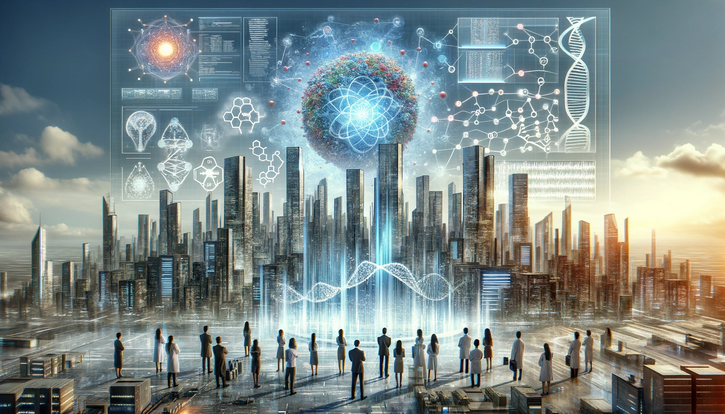
\includegraphics[width=0.5\textwidth]{figures/dall-e.png}
        \caption{Imagen generada con DALL-E 3.}
        \label{fig:dall-e}
    \end{figure}
\end{comment}

Si bien existen diversas formas de clasificar la IA, una de las más interesantes respecto a este PFG es la basada en la representación y el procesamiento del conocimiento. Según esta clasificación, existen dos tipos: la simbólica y la subsimbólica. La IA simbólica utiliza representaciones explícitas y legibles para los humanos, como símbolos y reglas lógicas, para resolver problemas. Consiste en incorporar conocimientos humanos y reglas de comportamiento a programas informáticos. Por otro lado, la subsimbólica se centra en métodos que no dependen de representaciones explícitas y se inspiran en los procesos naturales.

En las últimas décadas, la IA subsimbólica ha sido la más desarrollada, destacándose en tres campos principalmente.

Primero, el aprendizaje automático, particularmente a través de redes neuronales, que permite aprender y procesar grandes volúmenes de datos. Un ejemplo de esto es el proyecto \textit{AlphaFold} de \textit{DeepMind}, que utiliza IA para predecir las estructuras de proteínas, acelerando la investigación científica en la creación de nuevos medicamentos~\cite{alphafold2024}.

El segundo es la lógica borrosa, que simula la forma en la que los humanos toman decisiones en situaciones de incertidumbre. Un ejemplo interesante de esto es su uso en la industria automotriz para mejorar la estabilidad del vehículo mediante la regulación adaptativa de los amortiguadores en respuesta a las condiciones de la carretera y las dinámicas del vehículo~\cite{ivanov2015}.

Por último, la computación evolutiva, que emplea procesos evolutivos biológicos para la resolución de problemas. Dentro de esta rama destacan principalmente dos tipos de algoritmos.

Uno de ellos son los algoritmos de enjambre. Inspirados en el comportamiento colectivo de sistemas naturales como colonias de hormigas o bandadas de aves, son métodos de optimización que solucionan problemas complejos mediante la colaboración de múltiples agentes simples. Un uso actual destacado de estos algoritmos es en la optimización de granjas eólicas, donde se emplean para mejorar la ubicación de turbinas y maximizar la eficiencia energética~\cite{dong2023}.

La otra categoría son los algoritmos evolutivos, foco principal de este proyecto. Basados en la teoría de la evolución, aplican procesos como selección y mutación para mejorar iterativamente soluciones hasta alcanzar un objetivo.

\section{Algoritmos evolutivos}

Un algoritmo se puede definir como un procedimiento computacional bien definido que toma un valor, o un conjunto de valores, como entrada y produce un valor, o un conjunto de valores, como salida. Se trata de un conjunto de instrucciones que permiten realizar una actividad mediante sucesivos pasos.

Un algoritmo evolutivo es un tipo de algoritmo que proviene de la computación evolutiva. Esta rama de la IA emplea principios inspirados en la evolución biológica para la resolución de problemas. Teoría propuesta por Charles Darwin en 1859~\cite{darwin1859}, expone que en la naturaleza, en un entorno dado que puede albergar un número limitado de individuos, la selección natural favorece a aquellos que poseyeran características que les permitiesen adaptarse mejor al medio, teniendo una mayor posibilidad de sobrevivir y reproducirse. A lo largo del tiempo, las características ventajosas se propagan a través de las generaciones, mientras que aquellas menos favorables tienden a desaparecer. Por lo tanto, estas poblaciones irán evolucionando y adaptándose gradualmente al entorno.

Los algoritmos evolutivos han tenido varios proyectos que han marcado el desarrollo de esta tecnología. Los primeros acercamientos tuvieron lugar en las décadas de 1960 y 1970. Por un lado, Lawrence J. Fogel (1966)~\cite{fogel1966} comenzó a explorar la programación evolutiva, centrándose en la evolución de autómatas finitos. Fue uno de los primeros intentos de aplicar principios evolutivos a la informática. Por otro lado, Rechenberg (1973)~\cite{rechenberg1973} desarrolló estrategias de evolución para problemas de optimización. Centradas en la selección y en la mutación, resultaron ser muy útiles para aplicarlas en la realidad.

Tras estos primeros pasos, John Holland fue fundamental para el desarrollo de los algoritmos genéticos (AGs), subrama que se inspira en la genética para la optimización de problemas. Su libro \textit{''Adaptation in Natural and Artificial Systems''} (1975)~\cite{holland1975} se centró en la idea de que la evolución biológica podía ser simulada y utilizada para resolver problemas complejos en computación. Como se observa en el listado \ref{lst:algoritmo}, estos algoritmos hacen uso de la selección, el cruce o la mutación para evolucionar una población candidata de individuos hacia una mejor solución. Cada solución es evaluada según una función de fitness, que mide qué tan buena es la solución al problema en cuestión.
\newpage
\begin{lstlisting}[caption=Algoritmo evolutivo., label={lst:algoritmo}]
INICIAR
    INICIALIZAR población
    EVALUAR fitness
    REPETIR HASTA CUMPLIR condición de parada:
        SELECCIONAR individuos
        CRUZAR padres
        MUTAR hijos
        EVALUAR individuos
        FORMAR nueva generación
    RETORNAR solución
FINALIZAR
\end{lstlisting}

Para que un AG se vaya reconduciendo hacia soluciones más favorables, se hace uso de las restricciones. Se usan diversas técnicas, como penalizar las soluciones que violan las restricciones, emplear métodos de reparación para modificar las soluciones no válidas o descartar directamente las soluciones que no sean factibles. Estas estrategias permiten que los algoritmos genéticos mantengan la diversidad de la población a la vez que mejora la convergencia hacia una solución válida.

Después de que Holland sentara las bases de los algoritmos genéticos, en los años siguientes fueron surgiendo estudios que hicieron evolucionar la rama. Varios de los más importantes fueron de John Koza~\cite{koza1992}~\cite{koza1994}, quien introdujo la programación genética, técnica usada para desarrollar automáticamente programas que realicen una tarea definida por el usuario. Se optimiza una población de individuos (programas) respecto a una función de aptitud. Koza probó su viabilidad para resolver problemas de robótica o de optimización.

Tras él han seguido surgiendo nuevas técnicas dentro de los algoritmos evolutivos. Entre ellas se puede destacar el desarrollo de la \textit{Programación genética cartesiana (CGP)}, que sustituye los árboles de búsqueda usados en la programación genética tradicional por grafos dirigidos acíclicos, lo cual es muy útil, por ejemplo, en el diseño de circuitos electrónicos~\cite{miller2000}.

Otro avance que se ha popularizado es el de los \textit{Algoritmos genéticos híbridos (AGHs)}, que combinan los algoritmos genéticos con otras técnicas de optimización para mejorar las soluciones a los problemas complejos.\newpage En esta subrama destacan los algoritmos meméticos. Estos combinan algoritmos evolutivos con búsqueda local para mejorar la calidad y velocidad de convergencia de las soluciones. Después del cruce y de la mutación, cada nueva solución se refina explorando soluciones cercanas para encontrar mejoras.~\cite{moscato2003}

A lo largo de los años se han desarrollado distintos proyectos pioneros que han hecho uso de los algoritmos genéticos. Se puede destacar la misión de la NASA \textit{Space Technology 5 (ST5)}, donde ayudaron a la creación de una antena ultracompacta, con resultados extraordinarios~\cite{nasa2006}~\cite{lohn2004}. También han sido empleados en áreas tan diversas como la economía o la bioingeniería, donde pueden ayudar en tareas tan diversas como predecir movimientos del mercado~\cite{abraham2022} o a modelar secuencias genéticas~\cite{notredame1996}, respectivamente.

\section{Planificación nutricional mediante algoritmos evolutivos}

Los primeros acercamientos para intentar resolver problemas de optimización nutricional se dan en la década de 1940. George Stigler (1945)~\cite{stigler1945} planteó el problema de encontrar la dieta de menor coste que cumpliese con unos objetivos nutricionales. Al no poseer ordenadores, utilizó técnicas manuales.

El problema fue resuelto dos años después por Jack Laderman (1947)~\cite{problemasdedietas} usando programación lineal. Fue capaz de calcular la combinación de alimentos que cumpliese con los requisitos económicos y nutricionales. Con esto se demostró la utilidad de técnicas computacionales en tareas de optimización.

Tras los estudios de Holland, en las siguientes décadas aparecieron distintos trabajos que hacían uso de los algoritmos genéticos. Si bien estos no estaban relacionados directamente con la planificación nutricional, sí que sentaron las bases para la resolución de problemas de optimización. Se puede destacar los trabajos de Scott Kirkpatrick et al. (1983)~\cite{kirkpatrick1983} y de David E. Goldberg (1989)~\cite{goldberg1989}.

Fue a partir de la década de los 2000 cuando aparecieron muchos de los trabajos y estudios relacionados con la planificación nutricional.

El trabajo de Kahraman y Seven (2005)~\cite{kahraman2005} desarrolla un algoritmo genético bi-objetivo que propone comidas diarias saludables donde los parámetros son especificados por el usuario a través de la interfaz gráfica, como la edad o el género. Optimiza la selección de platos para cumplir con restricciones nutricionales, minimizar costos y maximizar las preferencias del usuario.

Kaldirim y Köse (2006)~\cite{kaldirim2006} hacen una continuación de este trabajo. Hace uso del algoritmo multiobjetivo NSGA-II para gestionar de manera separada los objetivos de coste mínimo y máxima satisfacción del usuario, mejorando el manejo de restricciones nutricionales con la inclusión de límites. También presenta una mejora a la interfaz gráfica del anterior proyecto.

El estudio de Kashima et al. (2009)~\cite{kashima2009} presenta una interesante diferencia respecto a trabajos anteriores. Busca crear una aplicación web para ofrecer un servicio para compartir menús, creados para cada individuo mediante algoritmos genéticos, entre una comunidad de usuarios cuyo objetivo es fomentar los hábitos saludables.

Heinonen y Juuso (2016)~\cite{heinonen2016} presentan el uso que le dan a los algoritmos genéticos en su aplicación Nutri-Flow, un software que proporciona guías dietéticas personalizadas. Emplea un sistema experto difuso \textit{(Fuzzy Expert System, FES)} junto con algoritmos genéticos para optimizar las recomendaciones. El FES evalúa los alimentos según sus características nutricionales y su contribución a las necesidades dietéticas individuales, mientras que los AGs buscan la combinación óptima de estos alimentos para ajustar la ingesta diaria.

En el trabajo realizado por Kilicarslan et al. (2021)~\cite{kilicarslan2021} se propone un modelo híbrido que combina algoritmos genéticos con aprendizaje profundo para la predicción y clasificación de anemias nutricionales. Optimiza los parámetros de los algoritmos de aprendizaje mediante computación evolutiva, mejorando así la precisión de la planificación nutricional del paciente.

Joanne B. Cole y Rosita Gabbiannelli (2022)~\cite{cole2022} muestran cómo se puede integrar la IA con el análisis genético para la nutrición personalizada del paciente. Basándose en el perfil genético y otros datos biométricos, es posible, junto a los algoritmos evolutivos, generar planes de comida y predicciones sobre la salud del usuario.